% \iffalse
\let\negmedspace\undefined
\let\negthickspace\undefined
\documentclass[journal,12pt,onecolumn]{IEEEtran}
\usepackage{cite}
\usepackage{amsmath,amssymb,amsfonts,amsthm}
\usepackage{algorithmic}
\usepackage{graphicx}
\usepackage{textcomp}
\usepackage{xcolor}
\usepackage{txfonts}
\usepackage{listings}
\usepackage{enumitem}
\usepackage{mathtools}
\usepackage{gensymb}
\usepackage{comment}
\usepackage[breaklinks=true]{hyperref}
\usepackage{tkz-euclide} 
\usepackage{listings}
\usepackage{gvv}                                        
\def\inputGnumericTable{}                                 
\usepackage[latin1]{inputenc}                                
\usepackage{color}                                            
\usepackage{array}                                            
\usepackage{longtable}                                       
\usepackage{calc}                                             
\usepackage{multirow}                                         
\usepackage{hhline}                                           
\usepackage{ifthen}                                           
\usepackage{lscape}
\usepackage{siunitx}
\usepackage{flushend}
\usepackage[siunitx]{circuitikz}
\usepackage{caption}
\usepackage{subcaption}

\newtheorem{theorem}{Theorem}[section]
\newtheorem{problem}{Problem}
\newtheorem{proposition}{Proposition}[section]
\newtheorem{lemma}{Lemma}[section]
\newtheorem{corollary}[theorem]{Corollary}
\newtheorem{example}{Example}[section]
\newtheorem{definition}[problem]{Definition}
\newcommand{\BEQA}{\begin{eqnarray}}
	\newcommand{\EEQA}{\end{eqnarray}}
\newcommand{\define}{\stackrel{\triangle}{=}}
\theoremstyle{remark}
\newtheorem{rem}{Remark}
\begin{document}
	
	\bibliographystyle{IEEEtran}
	\vspace{3cm}
	
	\title{NCERT 12.7 Q.13}
	\author{EE23BTECH11203 - Adarsh A$^{*}$% <-this % stops a space
	}
	\maketitle
	%\newpage
	\bigskip
	
	\renewcommand{\thefigure}{\theenumi}
	\renewcommand{\thetable}{\theenumi}


	\vspace{0.2cm}
	\linespread{1}
	
	
	\textbf{\fontsize{13}{20}\selectfont 
		{Question : }} \fontsize{13}{20}\selectfont A coil of inductance 0.50 H and resistance 100 $\Omega$ is connected to a
		240 V, 50 Hz ac supply.
		
		(a) What is the maximum current in the coil?
		
	    (b) What is the time lag between the voltage maximum and the
		current maximum?
		
	\vspace{0.3cm}
	
	\begin{table}[htbp]
	\centering
	\noindent
	%\small
	\resizebox{0.5\textwidth}{!}{%
		\begin{tabular}{|c|c|c|}
			\hline
			\textbf{\fontsize{7.5}{20}\selectfont{Parameter}} &
			\textbf{\fontsize{7.5}{20}\selectfont{Value}} &
			\textbf{\fontsize{7.5}{20}\selectfont{Description}}\\
			
			\hline
			\fontsize{7.5}{20}\selectfont{V$_{rms}$} &
			\fontsize{7.5}{20}\selectfont{240 V} &
			\fontsize{7.5}{20}\selectfont{Effective voltage} \\
			\hline
			\fontsize{7.5}{20}\selectfont{f} &
			\fontsize{7.5}{20}\selectfont{50 \si{\hertz}} &
			\fontsize{7.5}{20}\selectfont{Oscillations per unit time} \\
			\hline
			\fontsize{7.5}{20}\selectfont{R} &
			\fontsize{7.5}{20}\selectfont{100 \si{\ohm}} &
			\fontsize{7.5}{20}\selectfont{Resistance} \\
			\hline
			\fontsize{7.5}{20}\selectfont{L} &
			\fontsize{7.5}{20}\selectfont{0.50 H} &
			\fontsize{7.5}{20}\selectfont{Inductance} \\
			\hline
			\fontsize{7.5}{20}\selectfont{$\phi$} &
			\fontsize{7.5}{20}\selectfont{-} &
			\fontsize{7.5}{20}\selectfont{Phase difference} \\
			\hline
			\fontsize{7.5}{20}\selectfont{$t_1$} &
			\fontsize{7.5}{20}\selectfont{-} &
			\fontsize{7.5}{20}\selectfont{Time of V$_{max}$} \\
			\hline
			\fontsize{7.5}{20}\selectfont{$t_2$} &
			\fontsize{7.5}{20}\selectfont{-} &
			\fontsize{7.5}{20}\selectfont{Time of I$_{max}$} \\
			\hline
			\fontsize{7.5}{20}\selectfont{$\Delta t$} &
			\fontsize{7.5}{20}\selectfont{$t_2$ - $t_1$} &
			\fontsize{7.5}{20}\selectfont{Time lag} \\
			\hline
		\end{tabular}
	}

	\hspace{3cm}
	\caption*{Input Table}
	
\end{table}
	
	\solution
		
	\begin{figure}[htbp]
		\centering
		\begin{circuitikz} \draw
			
			(2,0) to[sinusoidal voltage source, l=240<\volt>][i_=I A] (8,0)
			(2,0) to (2,3) to (3,3)
			(3,3) to[resistor, l=100 \ohm] (5,3)
			(5,3) to[inductor, l=0.50 <\henry>] (8,3) to (8,0)
			;
			
		\end{circuitikz}
		\caption*{Given Circuit}
	\end{figure}
	\begin{figure}[htbp]
		\centering
		\begin{circuitikz} \draw
			
			(2,0) to[sinusoidal voltage source, l=V(s)][i_=I(s)] (8,0)
			(2,0) to (2,3) to (3,3)
			(3,3) to[resistor, l=R] (5,3)
			(5,3) to[inductor, l=sL] (8,3) to (8,0)
			;
			
		\end{circuitikz}
		\caption*{s-domain Circuit}
	\end{figure}

	\textbf{(a)} Peak voltage is given as,
	\begin{align}
		V_0 &= \sqrt{2} V_{rms}\\
			&= 240\sqrt{2} \hspace{2pt} V
	\end{align}
	
	Angular frequency is,
	\begin{align}
		\omega &= 2\pi f \\
			&= 100\pi \hspace{3pt} rad/sec
	\end{align}
	
	Magnitude of total impedance is,
	\begin{align}
		Z &= \sqrt{R^2 + (\omega L)^2}\\ 
		&= \sqrt{(100)^2 + (50\pi)^2}\\
		&= 186.21 \hspace{3pt}\Omega
	\end{align}
	
	Now, maximum current is given by Ohm's law,
	\begin{align}
		I_{max} &= \dfrac{V_0}{Z}\\[3pt]
		&= \dfrac{240\sqrt{2}}{186.21}\\[3pt] 
		I_{max} &= 1.82 \hspace{3pt} Amp
	\end{align}
	
	$\therefore$ \hspace{0.2cm} The maximum current is 1.82 Amperes
	\vspace{0.5cm}
	
	\textbf{(b)} Equation of voltage is given as,
	\begin{align}
		V &= V_0 \cos(\omega t)
	\end{align}

	Equation of current is given as,
	\begin{align}
		I &= I_0 \cos(\omega t - \phi)
	\end{align}
	
	Maximum is obtained when,
	\begin{align}
		V_{max} &= V_0 \cos \brak 0\\
		\implies \omega t_1 &= 0\\
		\implies t_1 &= 0
	\end{align}
	
	Similarly,
	\begin{align}
		I_{max} &= I_0 \cos \brak 0\\
		\implies \omega t_2 - \phi  &= 0\\
		\implies t_2 &= \dfrac{\phi}{\omega}
	\end{align}
	
	Phase angle is given by the relation,
	\begin{align}
		\tan \phi &= \dfrac{\omega L}{R}\\[6pt]
		&= \dfrac{50 \pi}{100}\\[6pt]
		\phi &= \dfrac{57.5 \pi}{180} \hspace{3pt} rad
	\end{align}
	
	Time lag,
	\begin{align}
		\Delta t &= t_2 - t_1\\[5pt]
			&= \dfrac{\phi}{\omega} - 0\\[5pt]
			&=  \dfrac{57.5 \pi}{(180)(100 \pi)}\\[5pt]
		\Delta t &= 3.2 \hspace{3pt} ms
	\end{align}
	
	$\therefore$ \hspace{0.2cm}The time lag between maximum voltage and maximum current is 3.2 ms
	
	\vspace{0.3cm}
	\begin{figure}[htbp]
		\centering
		\begin{subfigure}{0.47\textwidth}
			\centering
			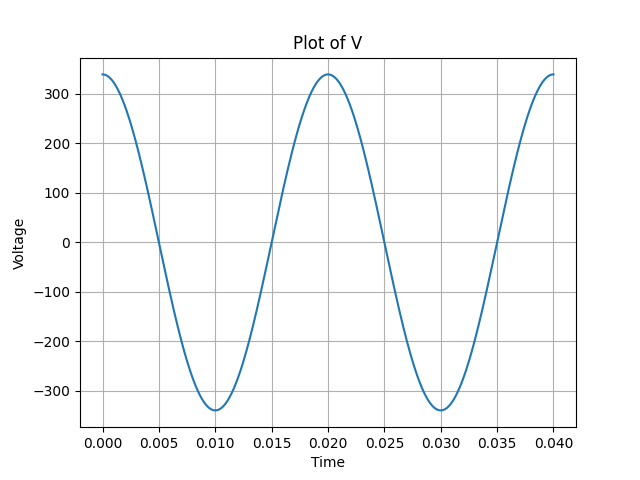
\includegraphics[width=\linewidth]{figs/Fig1.png}
			\caption{Plot of $V$ vs $t$}
		\end{subfigure}
		\hfill
		\begin{subfigure}{0.47\textwidth}
			\centering
			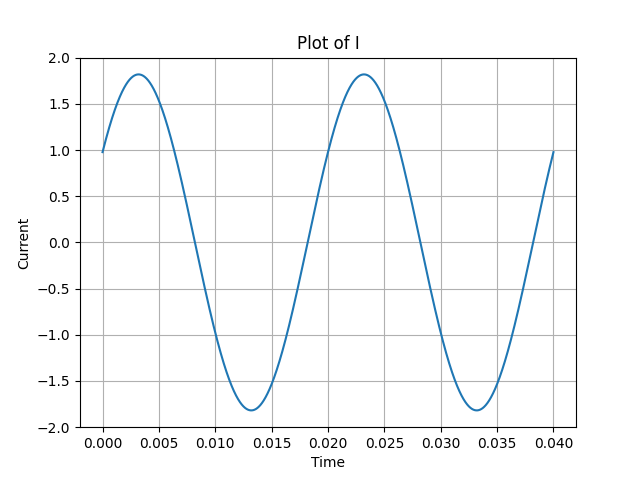
\includegraphics[width=\linewidth]{figs/Fig2.png}
			\caption{Plot of $I$ vs $t$}
		\end{subfigure}
	\end{figure}
	
	
\end{document}
